\documentclass[titlepage]{article}

%
% Geometry of the report (more spacing)
%
\usepackage[margin=3.5 cm]{geometry}

%
% Packages to use with report
%
\usepackage{url}
\usepackage{amsmath}
\usepackage{amsfonts}
\usepackage{subfig}
\usepackage{graphicx}

%
% Added math operators
%
\DeclareMathOperator*{\argmax}{arg\,max}
\DeclareMathOperator*{\argmin}{arg\,min}
\DeclareMathOperator{\var}{\mathrm{Var}}

%
% Author and title info
%
\author{Author Name}
\title{
    Main Title of the \LaTeX{} Document
    \\ \small \textbf{
        Possible Subtitle of \LaTeX{} Document
    }
}

%
% Document begin
%
\begin{document}

\maketitle

\section{Quadrature Phase-Shift Keying}
Fig.~\ref{fig:qpsk_constellation}a shows the four symbols used in QPSK modulation. The symbol values are given by 
$s_0 = \exp{(j\pi/4)}$, $s_1 = \exp{(j3\pi/4)}$, $s_2 = \exp{(j5\pi/4)}$ and $s_3 = \exp{(j7\pi/4)}$.
Fig.~\ref{fig:qpsk_constellation}b and 1c shows the received constellation of an AWGN channel feed with 100 random
QPSK symbols, with noise variance 0.01 (b) and 1.00 (c).

\begin{figure}
    \centering
    \subfloat[][] {
        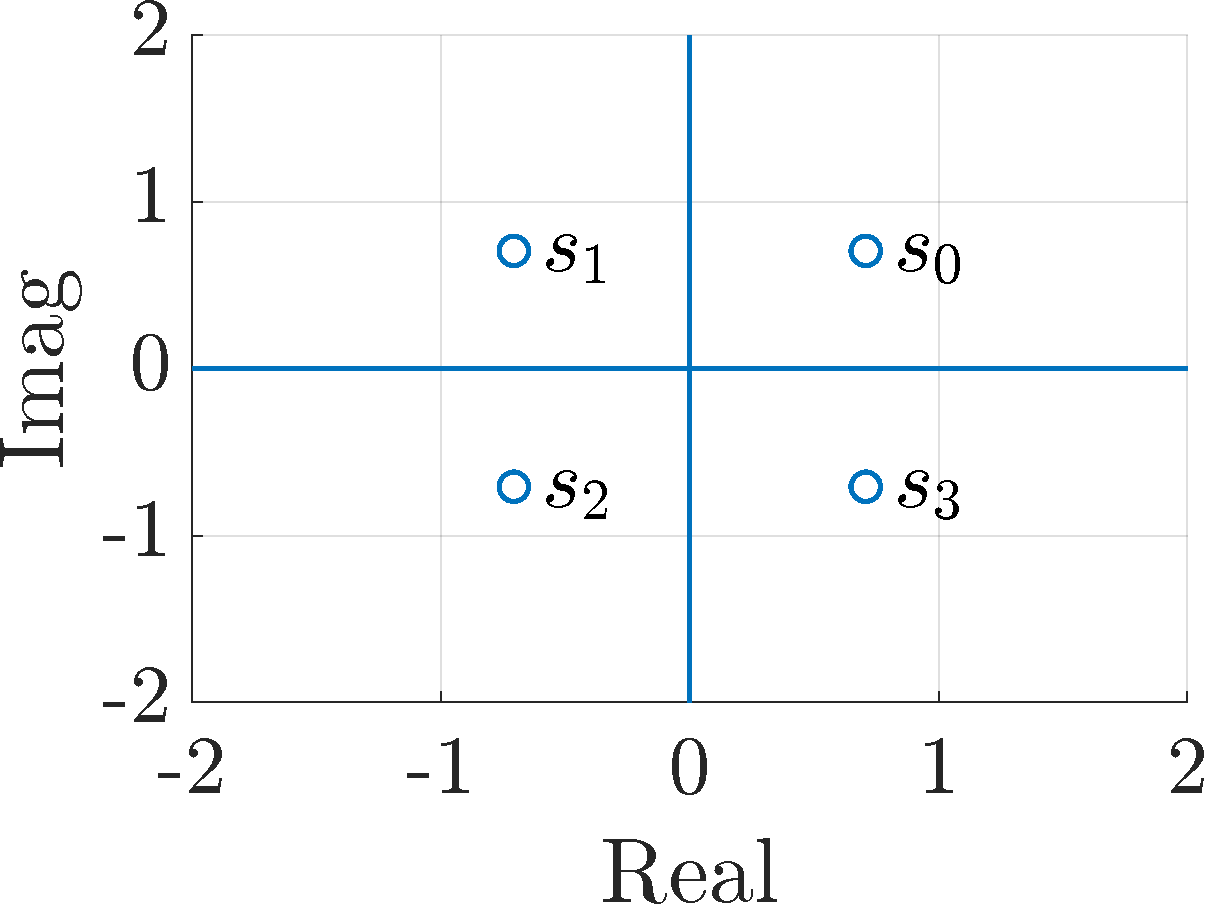
\includegraphics[width=0.3\textwidth]{figures/QPSK-Constellation.pdf}
        \label{fig:constellation:bpsk}
    }
    \subfloat[][] {
        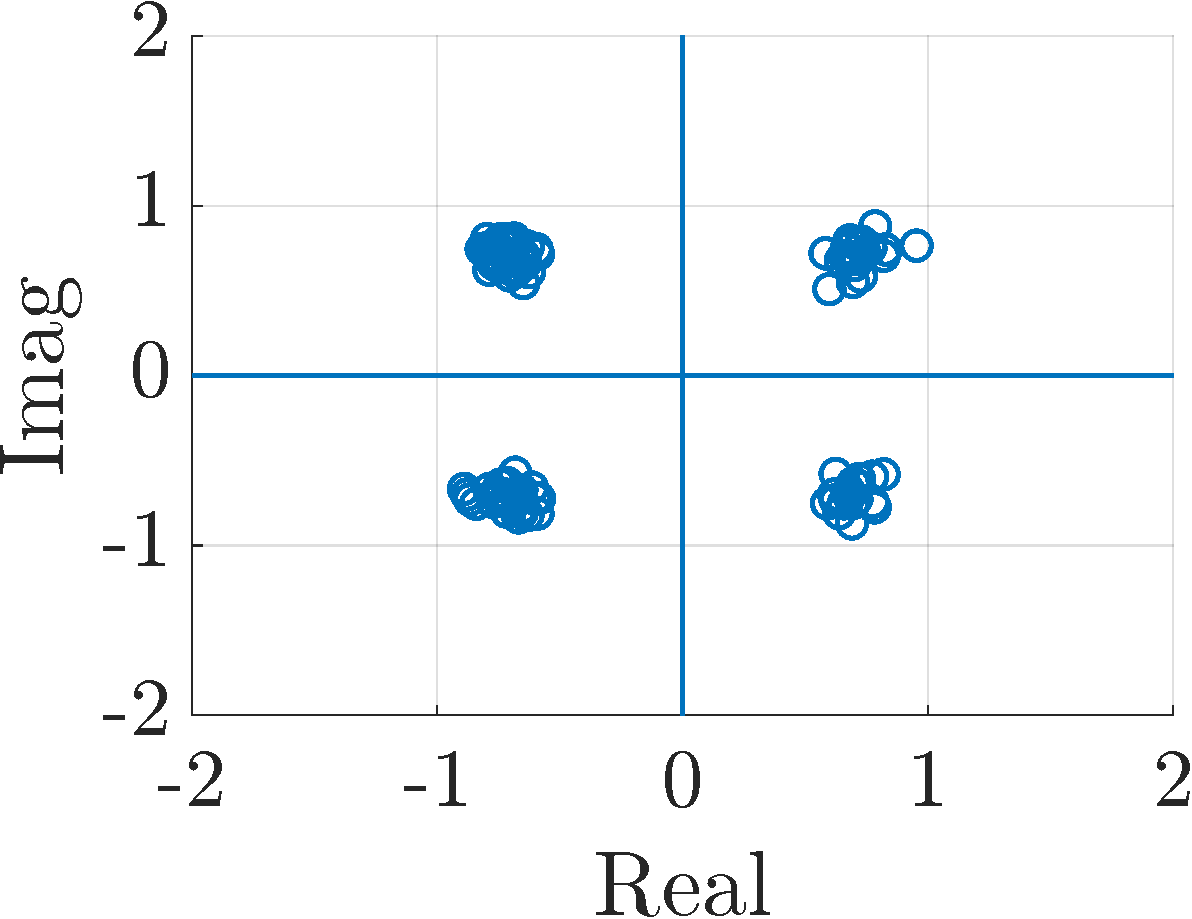
\includegraphics[width=0.3\textwidth]{figures/QPSK-AWGN-Noise1.pdf}
        \label{fig:constellation:qpsk}
    }
    \subfloat[][] {
        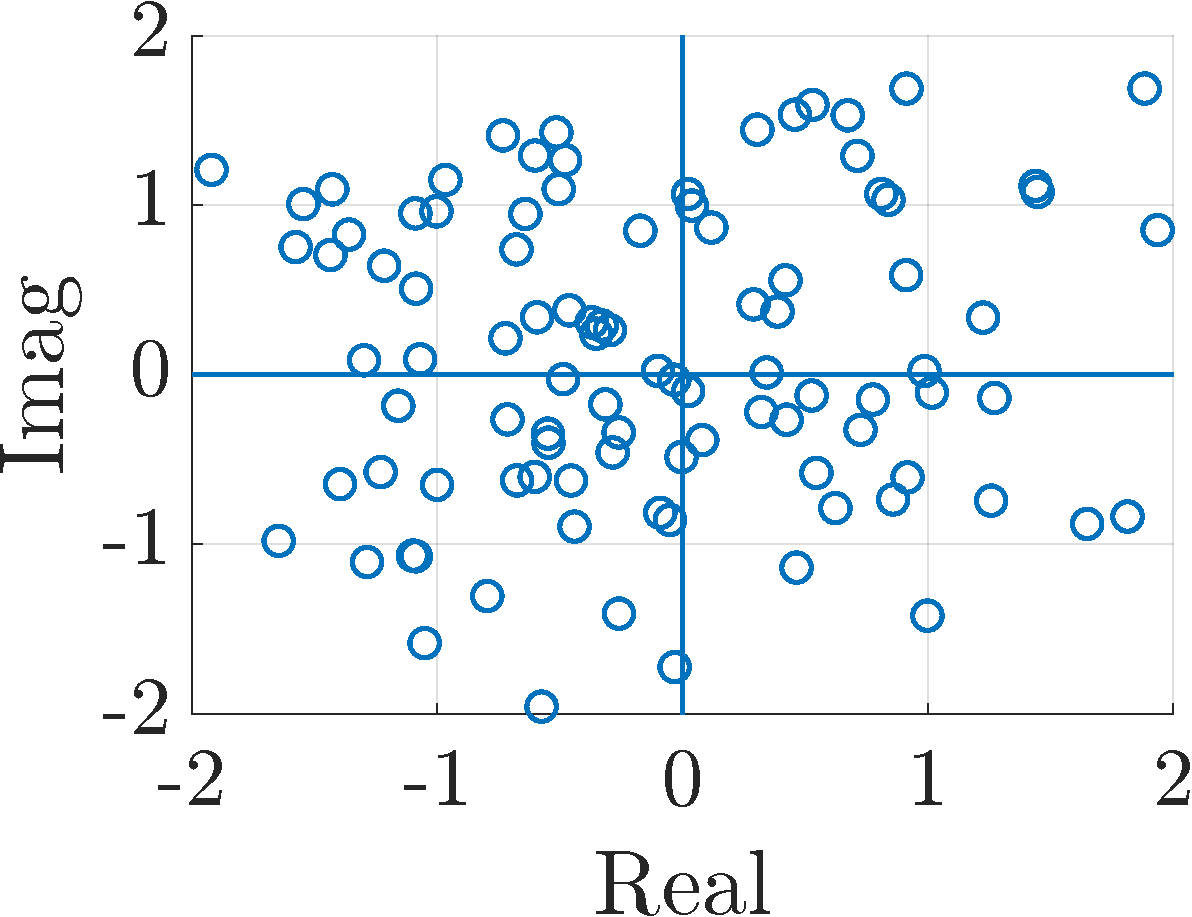
\includegraphics[width=0.3\textwidth]{figures/QPSK-AWGN-Noise2.pdf}
        \label{fig:constellation:qpsk}
    }
    \caption{
        Constellation diagram showing: 
        (a) the QPSK modulation symbols,
        (b) 100 QPSK modulated symbols over an AWGN channel with noise variance 0.01, and
        (c) 100 QPSK modulated symbols over an AWGN channel with noise variance 1.00.
    }
    \label{fig:qpsk_constellation}
\end{figure}

%
% Include the references
%
\bibliographystyle{ieeetr}
\bibliography{references}

\end{document}

